\section{Streaming Scheme}

Information processing tasks, such as classical compression gain a huge advantage implementing the process using a streaming scheme. Rather than start the compression on all the data to be sent and wait for it all to be compressed then send the data, as compression can be performed sequentially, compress part of the message and send it while compressing the next part. The Schur transform can also be thought of in this way. However, with compression it can still be useful to only compress part of the message, it is meaningless to perform only part of the Schur transform which suggests there may be a more optimal scheme opposed to streaming for implementing the Schur transform.      

The streaming Schur transform is described in \autoref{fig:stream},

\begin{figure}[h!]
\centering
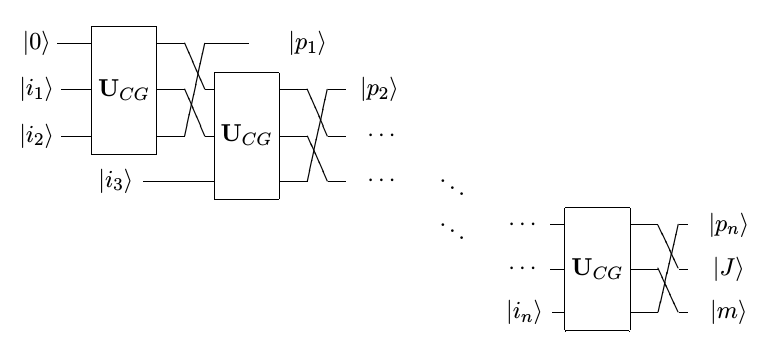
\includegraphics[width=0.6\textwidth]{schurcascade.png}
\caption{Streaming structure where the Schur transform is built up from consecutive Clebsch-Gordan transforms \cite{bacon2006efficient}.}
\label{fig:stream}
\end{figure}

The aim of this report is to look at whether it is possible to achieve a log decrease in time by instead of coupling 1 qubit in at a time to the $J$ \& $M$ registers, to pairing the couplings up in a \textbf{binary tree?} technique. To investigate the problem we look at how the complexity of performing the Clebsch-Gordan transform scales moving from coupling a single qubit to an arbitrary $J \& M$ to coupling arbitrary $J \& M$ registers together. looking at the pairing approach there is a symmetry in the fact that the max range of $J \& M$ values will be the same within each pairing which will help simplify the problem compared to any arbitrary $J \& M$ values.

For the streaming scheme the $U_{CG}$ block can be chosen so that it contains all of the gates for upto the n-th qubit meaning the same block can be repeated. 
Where the $U_{CG}$ is the Clebsch-Gordan transform between the $J$ \& $M$ registers and the k-th qubit $\ket{i_k}$.

\begin{figure}[h!]
\centering
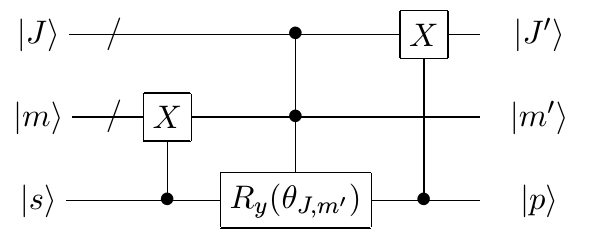
\includegraphics[width=0.6\textwidth]{genaddercirc.png}
\caption{$U_{CG}$ block, Qadder, controlled rotation, Qadder \cite{bacon2006efficient}.}
\label{fig:ucg}
\end{figure}

The controlled Rotation matrix, $R_y(\theta_{J,m'})$ \autoref{fig:stream} is the Clebsch-Gordan coefficients for coupling 1 qubit sequentially, given by,
\begin{align}
\begin{split}
R_y(\theta_{J,m'})=
\begin{bmatrix}
\cos(\theta_{J,m'}) &-\sin(\theta_{J,m'}) \\
\sin(\theta_{J,m'}) & \cos(\theta_{J,m'}) \\
\end{bmatrix}
\end{split}
=
\begin{split}
\frac{1}{\sqrt{2J+1}}
\begin{bmatrix}
\sqrt{J+\frac{1}{2}+m'} &-\sqrt{J+\frac{1}{2}-m'} \\
\sqrt{J+\frac{1}{2}-m'} & \sqrt{J+\frac{1}{2}+m'} \\
\end{bmatrix}
\end{split}
\label{eq:rotmatrix}
\end{align}

Where primed variables means after the angular momentum addition so $J$ is the total J that the spin is coupling to, the system will have $J'$ total angular momentum after the coupling. $m$ is the z component of the system before and $m'$ is the total z component after the coupling.

To build this circuit the rotation matrix, $R_y(\theta_{J,m'})$ needs to be calculated using \autoref{eq:rotmatrix}, values here \autoref{eq:rvalues}, and a function to update the $\ket{m}$ and $\ket{J}$ registers is needed. Updating the registers can be implemented relatively simply using the coherent (meaning the registers are allowed to be in superpositions) equivalent of the digital full adders and subtractors. The complexity now has been reduced to implementing the Clebsch-Gordan transform, $U_{CG}$.

\section{Implementing the Clebsch-Gordan Transform}

The vanilla transform directly maps the computation basis states to a labeling of J and M values. The vanilla approach of calculating the CG coefficients and finding a gate decomposition does not scale well. A better approach is to use a scheme explicitly storing the values of J \& M in registers.

The streaming scheme uses temporal multiplexing to perform the Schur transform in polynomial time if a recursive streaming scheme is used \cite{bacon2007quantum}.
